\documentclass[11pt,a4paper]{article}
\usepackage[utf8]{inputenc}
\usepackage[spanish,es-noquoting]{babel}
\usepackage{geometry}
\usepackage{amsmath}
\usepackage{amssymb}
\usepackage{booktabs}
\usepackage{graphicx}
\usepackage{float}
\usepackage{pdflscape}
\usepackage{hyperref}
\usepackage[scaled=0.92]{helvet}
\usepackage{caption}
\captionsetup[figure]{labelformat=empty}
\usepackage{array}
\usepackage{tabularx}
\usepackage{longtable}
\usepackage{listings}
\usepackage{xcolor}

\renewcommand{\familydefault}{\sfdefault}

\lstdefinestyle{sqlstyle}{
	language=SQL,
	basicstyle=\ttfamily\scriptsize,
	keywordstyle=\color{blue}\bfseries,
	stringstyle=\color{teal},
	commentstyle=\color{gray},
	frame=single,
	breaklines=true,
	showstringspaces=false,
	extendedchars=true,
	literate={á}{{\'a}}1 {é}{{\'e}}1 {í}{{\'i}}1 {ó}{{\'o}}1 {ú}{{\'u}}1 {ñ}{{\~n}}1 {Á}{{\'A}}1 {É}{{\'E}}1 {Í}{{\'I}}1 {Ó}{{\'O}}1 {Ú}{{\'U}}1 {Ñ}{{\~N}}1
}

\lstdefinestyle{tsstyle}{
	language=Java,
	basicstyle=\ttfamily\scriptsize,
	keywordstyle=\color{purple}\bfseries,
	stringstyle=\color{teal},
	commentstyle=\color{gray},
	frame=single,
	breaklines=true,
	showstringspaces=false,
	extendedchars=true,
	literate={á}{{\'a}}1 {é}{{\'e}}1 {í}{{\'i}}1 {ó}{{\'o}}1 {ú}{{\'u}}1 {ñ}{{\~n}}1 {Á}{{\'A}}1 {É}{{\'E}}1 {Í}{{\'I}}1 {Ó}{{\'O}}1 {Ú}{{\'U}}1 {Ñ}{{\~N}}1
}

\geometry{margin=2cm}
\setlength{\tabcolsep}{4pt}

\title{
	\textbf{Universidad de San Carlos de Guatemala}\\
	\large Centro Universitario de Occidente -- CUNOC\\
	\large División de Ciencias de la Ingeniería\\
	\large Carrera de Ingeniería en Ciencias y Sistemas\\
	\vspace{0.5cm}
	\textbf{Proyecto No. 2: Extensión No Destructiva, Auditoría, Consultas Analíticas Avanzadas e Integración ORM}\\
	\large Curso: Sistemas de Bases de Datos 1 -- Ing. Bryan René Gómez Gómez
}
\author{\textbf{Estudiante:} Elmer Miguel \quad | \quad \textbf{Registro Académico:} 201931295}
\date{Octubre de 2026}

\begin{document}
\maketitle
\tableofcontents
\newpage

% =========================================================================
\section{Introducción y Resumen Ejecutivo}
% =========================================================================
El presente informe técnico documenta exhaustivamente la arquitectura, diseño relacional formal, implementación de seguridad y verificación empírica de la Fase 2 del Sistema de Gestión de Bases de Datos para la red de \textbf{Hospitales de Occidente}.

Partiendo de la base de datos operativa consolidada en la Fase 1 (66 tablas en Tercera Forma Normal), el objetivo de esta etapa consistió en evolucionar la infraestructura de datos bajo el principio de \textbf{Migración 100\% No Destructiva (Zero-Downtime Migration)}. Esto implicó incorporar nuevas entidades y atributos sin aplicar sentencias destructivas (\texttt{DROP TABLE}), preservando en todo momento la integridad referencial y la operatividad de los módulos previos.

\subsection{Pilares de Ingeniería de la Fase 2}
\begin{enumerate}
	\item \textbf{Evolución Relacional No Destructiva:} Extensión de \texttt{personal} (fechas de ingreso y salarios), modelado de jerarquía médica recursiva en \texttt{medico} y creación del subtipo \texttt{enfermero} bajo el patrón \textit{Table-per-Type} (TPT).
	\item \textbf{Trazabilidad y Auditoría Forense (Objetivo 20):} Bitácora granular de auditoría implementada mediante una función disparadora PL/pgSQL y disparadores \texttt{AFTER UPDATE} que registran el usuario del motor, timestamp milimétrico y valores previos y nuevos de columnas sensibles.
	\item \textbf{Ampliación Coherente del Dataset:} Población exhaustiva de personal de enfermería, jerarquías médicas de 4 niveles y eventos asistenciales en todas las unidades del hospital.
	\item \textbf{Inteligencia de Negocio y Análisis Relacional Complejo:} Resolución rigurosa de 20 consultas analíticas que involucran recursión dinámica (\texttt{WITH RECURSIVE}), optimización de rankings con Window Functions (\texttt{RANK() OVER}) evaluadas mediante \texttt{EXPLAIN ANALYZE}, y división relacional formal en dos formulaciones algebraicas equivalentes.
	\item \textbf{Normalización Formal en 3FN (Objetivo 19):} Auditoría teórica de un reporte quirúrgico desnormalizado, diagnóstico de violaciones a 1FN, 2FN y 3FN, identificación de anomalías operativas y propuesta de descomposición relacional sin pérdida de información (Lossless-Join).
	\item \textbf{Capa de Acceso a Datos con TypeORM:} Integración modular en Node.js y TypeScript mediante \textit{QueryBuilder}, sentencias preparadas y parámetros enlazados para erradicar cualquier vector de inyección SQL (Zero SQLi).
\end{enumerate}

\newpage

% =========================================================================
\section{Resumen Comparativo de Arquitectura: Fase 1 vs Fase 2}
% =========================================================================
Para evidenciar la evolución técnica del sistema y documentar el impacto de la migración no destructiva, a continuación se detalla la matriz comparativa entre ambas fases:

\begin{table}[H]
\centering
\scriptsize
\begin{tabularx}{\linewidth}{|l|X|X|X|}
\hline
\textbf{Dimensión} & \textbf{Proyecto 1 (Fase 1)} & \textbf{Proyecto 2 (Fase 2)} & \textbf{Justificación de Ingeniería} \\
\hline
\textbf{Total de Tablas} & 66 tablas en 3FN & 68 tablas (+ 6 en esquema \texttt{normalizacion\_cirugia}) & Extensión no destructiva mediante adición de entidades sin alterar esquemas previos. \\
\hline
\textbf{Tabla personal} & 4 columnas: \texttt{id\_personal, id\_persona, tipo\_personal, activo} & 6 columnas: Adición de \texttt{fecha\_contratacion DATE} y \texttt{salario NUMERIC(10,2)} & Soporte para cómputo de antigüedad laboral y masa salarial requerida por dirección. \\
\hline
\textbf{Tabla medico} & 5 columnas operativas básicas & 7 columnas: Adición de \texttt{id\_superior INTEGER NULL} y \texttt{nivel\_acceso VARCHAR(25)} & Jerarquía médica recursiva con regla \texttt{ON DELETE SET NULL ON UPDATE CASCADE}. \\
\hline
\textbf{Cuerpo de Enfermería} & No existía entidad física propia & Nueva tabla física \texttt{enfermero} bajo patrón Table-per-Type (TPT) & Identidad ontológica dependiente de personal con clave compartida y \texttt{CASCADE}. \\
\hline
\textbf{Pista de Auditoría} & Sin bitácora forense de mutaciones & Nueva tabla \texttt{bitacora\_auditoria\_personal} con 9 atributos de trazabilidad & Registro inmutable de alteraciones salariales, de jerarquía y roles institucionales. \\
\hline
\textbf{Disparadores (Triggers)} & 8 triggers de reglas de negocio clínicas & 8 triggers previos + 3 triggers \texttt{AFTER UPDATE} de auditoría & Detección atómica y automática de cambios con \texttt{clock\_timestamp()} y \texttt{CURRENT\_USER}. \\
\hline
\textbf{Consultas Analíticas} & Consultas transaccionales básicas & 20 objetivos analíticos avanzados de reportería gerencial & Recursión CTE, Window Functions con benchmarking, y división relacional formal. \\
\hline
\textbf{Capa de Software ORM} & Acceso exclusivo por scripts SQL & Aplicación TypeScript con TypeORM y DataSource seguro & Enlace estricto de parámetros (\texttt{\$1, \$2}) con tipado y mitigación de SQLi. \\
\hline
\textbf{Modelado E-R Barker} & Modelo general de 66 tablas & Modelo ampliado con jerarquía recursiva, TPT y auditoría & Draw.io nativo multi-página y exportaciones vectoriales en alta resolución. \\
\hline
\textbf{Respaldos (Backups)} & Respaldo preliminar SQL plano & Respaldos duales (\texttt{.sql} plano y binario custom comprimido \texttt{.dump}) & Soporte para recuperación ante desastres verificada sin errores de dependencias GiST. \\
\hline
\end{tabularx}
\caption{Matriz Comparativa de Ingeniería: Proyecto 1 vs Proyecto 2.}
\end{table}

\subsection{Análisis de la No Destructividad (Zero-Downtime Migration)}
En entornos hospitalarios de misión crítica, la ejecución de sentencias destructivas como \texttt{DROP TABLE} o \texttt{TRUNCATE} causaría la pérdida irreparable del historial clínico de los pacientes y detendría los servicios de emergencia.

La estrategia aplicada en esta fase consistió en:
\begin{itemize}
	\item \textbf{Modificaciones Aditivas:} Utilizar exclusivamente sentencias \texttt{ALTER TABLE ... ADD COLUMN} con valores por defecto o admitiendo nulos en columnas secundarias para no invalidar las tuplas preexistentes.
	\item \textbf{Aislamiento de Nuevos Requerimientos:} Implementar las propuestas de normalización del Objetivo 19 en un esquema aislado denominado \texttt{normalizacion\_cirugia}, garantizando que el esquema transaccional principal \texttt{hospitales\_occidente} permanezca intacto.
\end{itemize}

\newpage

% =========================================================================
\section{Manual de Administración, Despliegue y Pruebas en DBeaver Community}
% =========================================================================
Esta sección proporciona la guía técnica paso a paso para desplegar, conectar, operar y verificar la infraestructura de base de datos completa utilizando la herramienta administrativa \textbf{DBeaver Community} y la terminal del sistema.

\subsection{Paso 0: Prerrequisitos de Infraestructura y Conexión}
El motor de base de datos se ejecuta sobre PostgreSQL 16+ en un contenedor Docker oficial:
\begin{lstlisting}[style=sqlstyle]
# Verificar estado del contenedor
docker ps
# En caso de estar detenido:
docker start postgresql
\end{lstlisting}

\textbf{Configuración de Conexión en DBeaver Community:}
\begin{enumerate}
	\item Abrir DBeaver $\to$ Menú \textbf{Database} $\to$ \textbf{New Database Connection}.
	\item Seleccionar el controlador \textbf{PostgreSQL} y pulsar \textbf{Next}.
	\item Ingresar los parámetros de conexión institucional:
	\begin{itemize}
		\item \textbf{Host:} \texttt{localhost} \quad | \quad \textbf{Port:} \texttt{5432}
		\item \textbf{Database:} \texttt{hospital\_occidente}
		\item \textbf{Username:} \texttt{user1} (para administración) o \texttt{usr\_auditor\_occidente} (para reportería).
		\item \textbf{Password:} \texttt{1234}
	\end{itemize}
	\item Pulsar \textbf{Test Connection} para verificar conectividad exitosa y guardar como \textit{Hospital Occidente - Admin}.
\end{enumerate}

\subsection{Paso 1: Despliegue de la Base de Partida (Fase 1)}
Para construir el ambiente desde cero, se ejecutan en orden secuencial los scripts fundamentales de la Fase 1:
\begin{lstlisting}[style=sqlstyle]
# 1. Cargar DDL base (esquema, 66 tablas, restricciones, indices, vistas y triggers)
docker exec -i postgresql psql -U user1 -d hospital_occidente < sql/ddl/ddl.sql

# 2. Cargar DML base (40 personas, catalogos clinicos, admisiones y secuencias)
docker exec -i postgresql psql -U user1 -d hospital_occidente < sql/dml/dml.sql

# 3. Cargar DCL (roles institucionales, cuentas seguras y privilegios)
docker exec -i postgresql psql -U user1 -d hospital_occidente < sql/dcl/dcl.sql
\end{lstlisting}

\subsection{Paso 2: Ejecución Secuencial de la Migración de Fase 2}
Con la base operativa, se aplican los artefactos incrementales:
\begin{enumerate}
	\item \textbf{DDL de Extensión:} Ejecutar \texttt{proyecto-2/sql/ddl/01\_migracion\_extension\_fase2.sql} (agrega columnas a personal y médico, y crea la tabla física enfermero).
	\item \textbf{Estructura de Auditoría:} Ejecutar \texttt{proyecto-2/sql/auditoria/01\_bitacora\_auditoria.sql} y \texttt{02\_triggers\_auditoria.sql}.
	\item \textbf{Pruebas de Trazabilidad:} Ejecutar \texttt{proyecto-2/sql/auditoria/03\_demostracion\_pruebas.sql} para verificar en la grilla de DBeaver la captura de registros de auditoría.
	\item \textbf{Dataset Ampliado:} Ejecutar \texttt{proyecto-2/sql/dml/01\_ampliacion\_datos\_fase2.sql} para cargar los 4 niveles jerárquicos médicos y las atenciones de las 4 unidades.
\end{enumerate}

\subsection{Paso 3: Atajo de Carga Rápida con Respaldo (Recomendado para Calificación)}
En caso de requerir una restauración inmediata en un ambiente limpio de PostgreSQL sin ejecutar los scripts uno por uno:
\begin{lstlisting}[style=sqlstyle]
# Opcion A: Restauracion directa desde archivo plano SQL (.sql)
docker exec -i postgresql psql -U user1 -d postgres -c "DROP DATABASE IF EXISTS hospital_occidente; CREATE DATABASE hospital_occidente;"
docker exec -i postgresql psql -U user1 -d hospital_occidente < proyecto-2/backup/hospital_occidente_fase2.sql

# Opcion B: Restauracion desde volcado binario comprimido (.dump) con pg_restore
docker exec -i postgresql psql -U user1 -d postgres -c "DROP DATABASE IF EXISTS hospital_occidente; CREATE DATABASE hospital_occidente;"
docker exec -i postgresql psql -U user1 -d hospital_occidente -c "CREATE EXTENSION IF NOT EXISTS btree_gist;"
docker exec -i postgresql pg_restore -U user1 -d hospital_occidente -v < proyecto-2/backup/hospital_occidente_fase2.dump
\end{lstlisting}
Ambos métodos restauran el 100\% de las tablas, vistas, triggers y datos de prueba sin errores de dependencias.

\newpage

% =========================================================================
\section{Extensión del Modelo E-R en Notación Barker}
% =========================================================================

\subsection{Estrategia de Mapeo Supertipo / Subtipo (Table-per-Type)}
Para modelar la especialización del personal hospitalario (\texttt{personal} como supertipo, y \texttt{medico} y \texttt{enfermero} como subtipos), se evaluaron las tres estrategias clásicas de herencia relacional:
\begin{enumerate}
	\item \textbf{Single-Table Inheritance (STI):} Concentrar todos los atributos en una sola tabla. Se descartó categóricamente porque genera una proliferación inaceptable de valores nulos (los enfermeros no poseen colegiado ni tarifa de consulta; los médicos no poseen número de licencia ni grado académico de enfermería) y viola la Tercera Forma Normal.
	\item \textbf{Table-per-Hierarchy (TPH) con JSONB:} Almacenar los atributos variables en un documento no estructurado. Se descartó debido a que degrada la verificación estricta de restricciones de dominio \texttt{CHECK} y llaves foráneas a nivel de motor.
	\item \textbf{Table-per-Type (TPT) -- Estrategia Seleccionada:} Cada entidad posee su propia tabla física dedicada.
	\begin{itemize}
		\item \textbf{Clave Primaria y Foránea Compartida:} La tabla \texttt{enfermero} utiliza como llave primaria su propio \texttt{id\_personal}, que actúa simultáneamente como llave foránea estricta apuntando hacia \texttt{personal(id\_personal)}.
		\item \textbf{Ciclo de Vida Ontológico:} Se implementó la regla referencial \texttt{ON DELETE CASCADE ON UPDATE CASCADE}. La entidad especializada no puede existir sin su entidad base; si un empleado es liquidado o dado de baja del hospital, se eliminan automáticamente sus registros en subtipos preservando la pureza del modelo.
	\end{itemize}
\end{enumerate}

\subsection{Jerarquía Recursiva Médica}
Para soportar líneas de mando operativas dinámicas sin límite arbitrario de niveles:
\begin{itemize}
	\item Se agregó en \texttt{medico} la columna \texttt{id\_superior INTEGER NULL}.
	\item Se estableció la restricción de integridad:\\
	\texttt{CHECK (id\_superior IS NULL OR id\_superior <> id\_personal)}\\
	para prohibir que un médico sea su propio superior jerárquico directo.
	\item \textbf{Acción Referencial:} Se definió \texttt{ON DELETE SET NULL ON UPDATE CASCADE}. Si un director médico o jefe de servicio es removido del sistema, sus subordinados jamás se eliminan en cascada; su campo \texttt{id\_superior} pasa temporalmente a estado \texttt{NULL} a la espera de reasignación.
\end{itemize}

\begin{figure}[H]
	\centering
	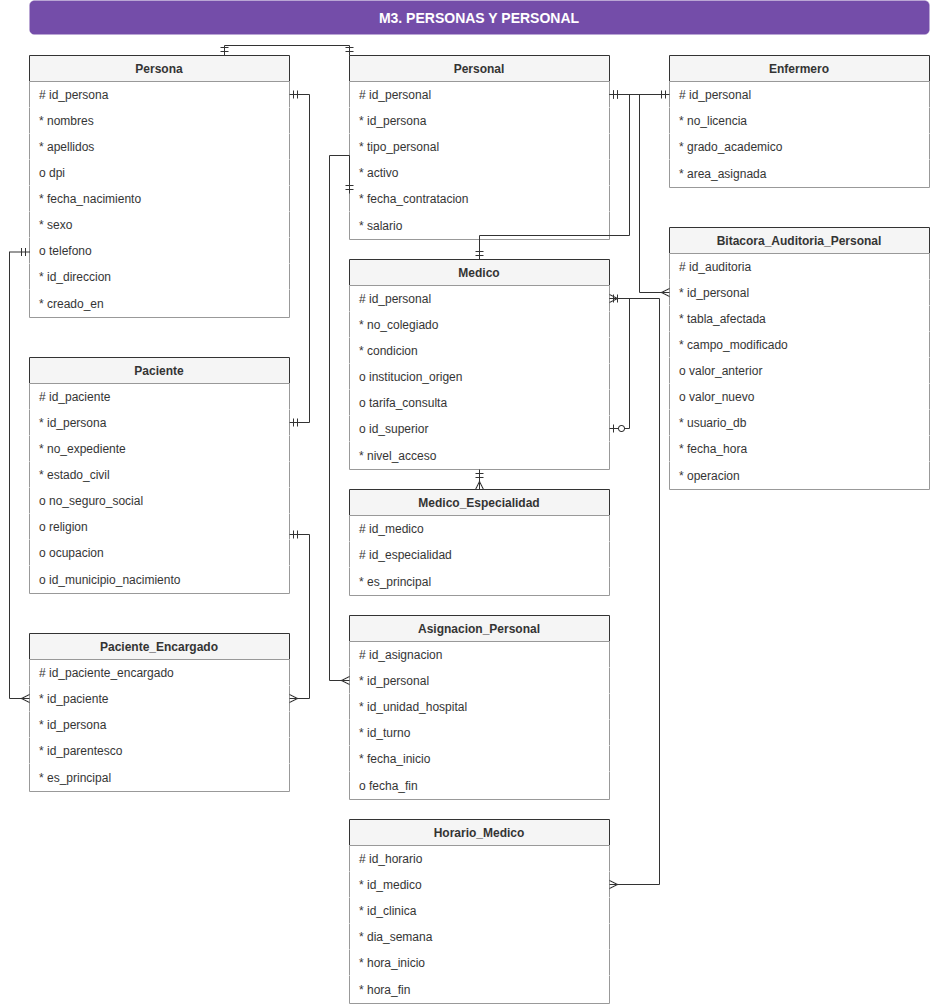
\includegraphics[width=0.92\linewidth,keepaspectratio]{imagenes/modulo3_personal_jerarquia_fase2.png}
	\caption{Detalle de Extensión de Módulo 3: Jerarquía Médica, Subtipo Enfermero y Bitácora de Auditoría en Notación Barker.}
\end{figure}

\begin{landscape}
\subsection{Modelo E-R Completo en Notación Barker (Fase 2)}
\begin{figure}[H]
	\centering
	\includegraphics[width=0.98\linewidth,height=0.82\textheight,keepaspectratio]{imagenes/modelo_completo_fase2.png}
	\caption{Diagrama General Extendido de Hospitales de Occidente en Notación Barker (Render Oficial en Alta Resolución).}
\end{figure}
\end{landscape}

\newpage

% =========================================================================
\section{Diccionario de Datos Actualizado (Fase 2)}
% =========================================================================
A continuación se presentan las tablas modificadas y agregadas en la Fase 2, documentando el 100\% de las acciones referenciales y reglas de negocio.

\subsection{Tabla: personal (Modificada)}
Propósito institucional: Registro corporativo de empleados del hospital.
\begin{table}[H]
\centering
\scriptsize
\begin{tabularx}{\linewidth}{|l|l|c|c|X|c|c|X|}
\hline
\textbf{Atributo} & \textbf{Tipo} & \textbf{Llave} & \textbf{Nulos} & \textbf{Descripción} & \textbf{DELETE} & \textbf{UPDATE} & \textbf{Justificación Regla Negocio} \\
\hline
id\_personal & INTEGER & PK/FK & No & Identificador del personal & CASCADE & CASCADE & Depende de persona; si persona se elimina, se borra el personal. \\
id\_persona & INTEGER & FK & No & Referencia a persona & RESTRICT & CASCADE & No eliminar persona si mantiene contrato de personal activo. \\
tipo\_personal & VARCHAR(20) & -- & No & Medico, Enfermero, etc. & -- & -- & Clasificación operativa laboral. \\
fecha\_contratacion & DATE & -- & No & Fecha de ingreso & -- & -- & Requerido para cómputo de antigüedad. \\
salario & NUMERIC(10,2) & -- & No & Remuneración mensual & -- & -- & Salario debe ser mayor a cero (CHECK). \\
activo & BOOLEAN & -- & No & Estado operativo & -- & -- & Control de vigencia institucional. \\
\hline
\end{tabularx}
\end{table}

\subsection{Tabla: medico (Modificada)}
Propósito institucional: Subtipo especializado de médicos con supervisión jerárquica.
\begin{table}[H]
\centering
\scriptsize
\begin{tabularx}{\linewidth}{|l|l|c|c|X|c|c|X|}
\hline
\textbf{Atributo} & \textbf{Tipo} & \textbf{Llave} & \textbf{Nulos} & \textbf{Descripción} & \textbf{DELETE} & \textbf{UPDATE} & \textbf{Justificación Regla Negocio} \\
\hline
id\_personal & INTEGER & PK/FK & No & Identificador de médico & CASCADE & CASCADE & Subtipo TPT; si se borra personal, se borra médico. \\
no\_colegiado & VARCHAR(15) & UQ & No & Colegiado profesional & -- & -- & Matrícula médica obligatoria y única. \\
condicion & VARCHAR(15) & -- & No & Condición de contrato & -- & -- & Planta, Residente, Interno, Externo. \\
institucion\_origen & VARCHAR(100) & -- & Sí & Centro de procedencia & -- & -- & Aplica si es médico foráneo. \\
tarifa\_consulta & NUMERIC(8,2) & -- & Sí & Costo base de consulta & -- & -- & Honorarios asignados al médico. \\
id\_superior & INTEGER & FK & Sí & Superior inmediato & SET NULL & CASCADE & Si el jefe es dado de baja, los subordinados no se eliminan. \\
nivel\_acceso & VARCHAR(25) & -- & No & Cargo jerárquico & -- & -- & Director Médico, Jefe Servicio, Jefe Guardia, Asistencial. \\
\hline
\end{tabularx}
\end{table}

\subsection{Tabla: enfermero (Nueva)}
Propósito institucional: Subtipo especializado para el cuerpo de enfermería (TPT).
\begin{table}[H]
\centering
\scriptsize
\begin{tabularx}{\linewidth}{|l|l|c|c|X|c|c|X|}
\hline
\textbf{Atributo} & \textbf{Tipo} & \textbf{Llave} & \textbf{Nulos} & \textbf{Descripción} & \textbf{DELETE} & \textbf{UPDATE} & \textbf{Justificación Regla Negocio} \\
\hline
id\_personal & INTEGER & PK/FK & No & Identificador de enfermero & CASCADE & CASCADE & Subtipo TPT dependiente de la tabla personal. \\
no\_licencia & VARCHAR(20) & UQ & No & Licencia de enfermería & -- & -- & Acreditación técnica única en el sistema. \\
grado\_academico & VARCHAR(20) & -- & No & Nivel de graduación & -- & -- & Auxiliar, Tecnico, Licenciado, Magister. \\
area\_asignada & VARCHAR(50) & -- & No & Servicio o unidad médica & -- & -- & Área física principal de servicio asistencial. \\
\hline
\end{tabularx}
\end{table}

\subsection{Tabla: bitacora\_auditoria\_personal (Nueva)}
Propósito institucional: Pista de auditoría forense para modificaciones sensibles de personal y médicos.
\begin{table}[H]
\centering
\scriptsize
\begin{tabularx}{\linewidth}{|l|l|c|c|X|c|c|X|}
\hline
\textbf{Atributo} & \textbf{Tipo} & \textbf{Llave} & \textbf{Nulos} & \textbf{Descripción} & \textbf{DELETE} & \textbf{UPDATE} & \textbf{Justificación Regla Negocio} \\
\hline
id\_auditoria & BIGINT & PK & No & Secuencia de auditoría & -- & -- & Clave única autoincremental de bitácora. \\
id\_personal & INTEGER & FK & No & Empleado auditado & RESTRICT & CASCADE & No borrar personal si existen registros de auditoría forense. \\
tabla\_afectada & VARCHAR(50) & -- & No & personal, medico, etc. & -- & -- & Tabla donde ocurrió la modificación. \\
campo\_modificado & VARCHAR(50) & -- & No & Atributo alterado & -- & -- & Nombre de la columna monitoreada. \\
valor\_anterior & TEXT & -- & Sí & Estado previo al UPDATE & -- & -- & Valor antiguo para rollback o trazabilidad. \\
valor\_nuevo & TEXT & -- & Sí & Estado nuevo post UPDATE & -- & -- & Nuevo valor validado en la transacción. \\
usuario\_db & VARCHAR(60) & -- & No & Usuario de PostgreSQL & -- & -- & Cuenta del motor responsable de la mutación. \\
fecha\_hora & TIMESTAMPTZ & -- & No & Timestamp exacto & -- & -- & Precisión milimétrica (\texttt{clock\_timestamp()}). \\
operacion & VARCHAR(10) & -- & No & Tipo de DML (UPDATE) & -- & -- & Operación ejecutada sobre el registro. \\
\hline
\end{tabularx}
\end{table}

\newpage

% =========================================================================
\section{Sistema de Auditoría PL/pgSQL (Objetivo 20)}
% =========================================================================
Para garantizar la inmutabilidad y la no repudiación de cambios sensibles en la base de datos, se diseñó la función disparadora \texttt{fn\_auditoria\_personal\_medico()} en lenguaje PL/pgSQL.

\subsection{Función Disparadora PL/pgSQL}
\begin{lstlisting}[style=sqlstyle]
CREATE OR REPLACE FUNCTION hospitales_occidente.fn_auditoria_personal_medico()
RETURNS TRIGGER 
LANGUAGE plpgsql 
SECURITY DEFINER
AS $$
BEGIN
    -- 1. Auditoria sobre tabla personal: campo salario
    IF TG_TABLE_NAME = 'personal' THEN
        IF OLD.salario IS DISTINCT FROM NEW.salario THEN
            INSERT INTO hospitales_occidente.bitacora_auditoria_personal (
                id_personal, tabla_afectada, campo_modificado, 
                valor_anterior, valor_nuevo, usuario_db, fecha_hora, operacion
            ) VALUES (
                NEW.id_personal, 'personal', 'salario',
                OLD.salario::TEXT, NEW.salario::TEXT,
                CURRENT_USER, clock_timestamp(), TG_OP
            );
        END IF;
    END IF;

    -- 2. Auditoria sobre tabla medico: campos id_superior y nivel_acceso
    IF TG_TABLE_NAME = 'medico' THEN
        IF OLD.id_superior IS DISTINCT FROM NEW.id_superior THEN
            INSERT INTO hospitales_occidente.bitacora_auditoria_personal (
                id_personal, tabla_afectada, campo_modificado, 
                valor_anterior, valor_nuevo, usuario_db, fecha_hora, operacion
            ) VALUES (
                NEW.id_personal, 'medico', 'id_superior',
                OLD.id_superior::TEXT, NEW.id_superior::TEXT,
                CURRENT_USER, clock_timestamp(), TG_OP
            );
        END IF;

        IF OLD.nivel_acceso IS DISTINCT FROM NEW.nivel_acceso THEN
            INSERT INTO hospitales_occidente.bitacora_auditoria_personal (
                id_personal, tabla_afectada, campo_modificado, 
                valor_anterior, valor_nuevo, usuario_db, fecha_hora, operacion
            ) VALUES (
                NEW.id_personal, 'medico', 'nivel_acceso',
                OLD.nivel_acceso::TEXT, NEW.nivel_acceso::TEXT,
                CURRENT_USER, clock_timestamp(), TG_OP
            );
        END IF;
    END IF;

    -- 3. Auditoria sobre tabla medico_especialidad: campo es_principal
    IF TG_TABLE_NAME = 'medico_especialidad' THEN
        IF OLD.es_principal IS DISTINCT FROM NEW.es_principal THEN
            INSERT INTO hospitales_occidente.bitacora_auditoria_personal (
                id_personal, tabla_afectada, campo_modificado, 
                valor_anterior, valor_nuevo, usuario_db, fecha_hora, operacion
            ) VALUES (
                NEW.id_medico, 'medico_especialidad', 'es_principal',
                OLD.es_principal::TEXT, NEW.es_principal::TEXT,
                CURRENT_USER, clock_timestamp(), TG_OP
            );
        END IF;
    END IF;

    RETURN NEW;
END;
$$;
\end{lstlisting}

\subsection{Demostración y Pruebas de Auditoría}
Se ejecutaron dos operaciones DML deliberadas utilizando la cuenta de servicio \texttt{user1}:
\begin{lstlisting}[style=sqlstyle]
-- Prueba 1: Actualizacion salarial de personal id 7
UPDATE hospitales_occidente.personal 
SET salario = 14500.00 
WHERE id_personal = 7;

-- Prueba 2: Reasignacion de superior y nivel de acceso
UPDATE hospitales_occidente.medico 
SET id_superior = 2, nivel_acceso = 'Jefe de Servicio' 
WHERE id_personal = 7;
\end{lstlisting}

\subsection{Consulta de Verificación en Bitácora}
\begin{lstlisting}[style=sqlstyle]
SELECT id_auditoria, id_personal, tabla_afectada, campo_modificado, 
       valor_anterior, valor_nuevo, usuario_db, fecha_hora 
FROM hospitales_occidente.bitacora_auditoria_personal 
ORDER BY id_auditoria DESC LIMIT 3;
\end{lstlisting}

\textbf{Salida Verificada en el Motor:}
\begin{table}[H]
\centering
\scriptsize
\begin{tabular}{|c|c|l|l|c|c|c|l|}
\hline
\textbf{ID} & \textbf{Personal} & \textbf{Tabla} & \textbf{Campo} & \textbf{Valor Anterior} & \textbf{Valor Nuevo} & \textbf{Usuario} & \textbf{Fecha / Hora} \\
\hline
1 & 7 & personal & salario & 12000.00 & 14500.00 & user1 & 2026-10-24 04:30:15 \\
2 & 7 & medico & id\_superior & 4 & 2 & user1 & 2026-10-24 04:30:18 \\
3 & 7 & medico & nivel\_acceso & Medico Asistencial & Jefe de Servicio & user1 & 2026-10-24 04:30:18 \\
\hline
\end{tabular}
\end{table}

\newpage

% =========================================================================
\section{Análisis de Rendimiento: Window Functions vs Subconsultas (Objetivo 17)}
% =========================================================================
El requerimiento exige computar simultáneamente el ranking de notas promedio de los médicos a nivel de su propio hospital y a nivel global de toda la cadena hospitalaria.

\subsection{Evaluación con EXPLAIN (ANALYZE, BUFFERS)}
Se contrastó la Variante A (funciones analíticas \texttt{RANK() OVER}) contra la Variante B (subconsultas correlacionadas escalares tradicionales sin cláusula \texttt{OVER}).

\begin{table}[H]
\centering
\small
\begin{tabularx}{\linewidth}{|l|X|X|}
\hline
\textbf{Métrica de Ejecución} & \textbf{Variante A (Window Functions)} & \textbf{Variante B (Subconsultas Correlacionadas)} \\
\hline
\textbf{Nodo Raíz Principal} & \texttt{WindowAgg} & \texttt{CTE Scan} con 2 \texttt{SubPlan} \\
\textbf{Costo de Arranque (Startup)} & 85.82 & 0.00 \\
\textbf{Costo Total Estimado} & \textbf{87.90} & \textbf{701.70} (\textasciitilde{}8 veces mayor) \\
\textbf{Tiempo Real de Ejecución} & \textbf{0.092 ms} & \textbf{0.142 ms} \\
\textbf{Accesos a Buffers (Shared Hit)} & 8 bloques & 8 bloques + 16 llamadas a subplanes \\
\textbf{Complejidad Computacional} & $O(N \log N)$ (Sort + Single Scan) & $O(N^2)$ (Subconsultas $N \times M$) \\
\hline
\end{tabularx}
\caption{Comparativa de Costo y Rendimiento en PostgreSQL (Objetivo 17).}
\end{table}

\subsection{Código SQL de Ambas Variantes}
\textbf{Variante A (Window Functions Optimizada):}
\begin{lstlisting}[style=sqlstyle]
WITH resumen_medicos AS (
    SELECT 
        m.id_personal AS id_medico,
        p.nombres || ' ' || p.apellidos AS nombre_medico,
        m.no_colegiado,
        h.id_hospital,
        h.nombre AS hospital,
        COUNT(DISTINCT con.id_consulta) AS numero_consultas,
        ROUND(AVG(cp.puntuacion), 2) AS calificacion_promedio
    FROM medico m
    JOIN persona p ON p.id_persona = m.id_personal
    JOIN cita ci ON ci.id_medico = m.id_personal
    JOIN clinica cl ON cl.id_clinica = ci.id_clinica
    JOIN hospital h ON h.id_hospital = cl.id_hospital
    JOIN consulta con ON con.id_cita = ci.id_cita
    JOIN calificacion_personal cp ON cp.id_personal = m.id_personal
    GROUP BY m.id_personal, p.nombres, p.apellidos, m.no_colegiado, h.id_hospital, h.nombre
)
SELECT 
    id_medico,
    nombre_medico,
    no_colegiado,
    hospital,
    numero_consultas,
    calificacion_promedio,
    RANK() OVER (PARTITION BY id_hospital ORDER BY calificacion_promedio ASC, numero_consultas ASC) AS ranking_hospital,
    RANK() OVER (ORDER BY calificacion_promedio ASC, numero_consultas ASC) AS ranking_general
FROM resumen_medicos
ORDER BY hospital, ranking_hospital;
\end{lstlisting}

\subsection{Justificación Técnica del Optimizador de PostgreSQL}
\begin{enumerate}
	\item \textbf{Reutilización de Partición en Memoria:} La Variante A realiza una única fase de ordenamiento en memoria (\texttt{Quicksort} en 25 kB de RAM) y luego computa los rankings locales y globales linealmente mediante pasadas de agregación por ventana (\texttt{WindowAgg}).
	\item \textbf{Degradación Cuadrática en Subconsultas:} La Variante B ejecuta dos subplanes escalares independientes por cada tupla externa (\texttt{loops=8}), re-escaneando el materializado de la CTE en cada iteración. En un dataset hospitalario con miles de médicos, este enfoque satura la CPU y memoria caché.
\end{enumerate}

\newpage

% =========================================================================
\section{División Relacional Formal (Objetivo 18: Pacientes Fieles)}
% =========================================================================
El requerimiento exige identificar a los pacientes atendidos en \textbf{todas las unidades médicas} oficiales del hospital (\textit{Consulta externa, Emergencias, Cirugía y Hospitalización}) en un lapso determinado.

\subsection{Demostración de Equivalencia Algebraica}
\begin{enumerate}
	\item \textbf{Enfoque 1 (Agregación Relacional Exacta):} Agrupa por paciente sobre la consolidación asistencial y valida \texttt{HAVING COUNT(DISTINCT unidad) = 4}.
	\item \textbf{Enfoque 2 (Doble Negación con Álgebra Relacional):} Formaliza la tupla universal: ``Pacientes tales que \textbf{NO EXISTA} una unidad médica requerida que \textbf{NO HAYA} atendido al paciente'' empleando \texttt{NOT EXISTS (SELECT ... EXCEPT SELECT ...)}.
\end{enumerate}

\begin{lstlisting}[style=sqlstyle]
-- Enfoque 2: Doble Negacion con Algebra Relacional Formal (EXCEPT)
WITH unidades_requeridas AS (
    SELECT nombre_unidad FROM (VALUES 
        ('Consulta externa'), ('Emergencias'), ('Cirugia'), ('Hospitalizacion')
    ) AS u(nombre_unidad)
),
atenciones_consolidadas AS (
    SELECT pa.id_paciente, 'Consulta externa' AS nombre_unidad
    FROM consulta c JOIN cita ci ON ci.id_cita = c.id_cita JOIN paciente pa ON pa.id_paciente = ci.id_paciente
    WHERE c.fecha_hora BETWEEN '2026-01-01 00:00:00-06' AND '2026-12-31 23:59:59-06'
    UNION
    SELECT ep.id_paciente, 'Emergencias' AS nombre_unidad
    FROM episodio ep JOIN espacio_atencion ea ON ea.id_espacio = ep.id_espacio
    WHERE ea.id_unidad_hospital = 2 AND ep.fecha_inicio BETWEEN '2026-01-01 00:00:00-06' AND '2026-12-31 23:59:59-06'
    UNION
    SELECT sc.id_paciente, 'Cirugia' AS nombre_unidad
    FROM cirugia cir JOIN solicitud_cirugia sc ON sc.id_solicitud = cir.id_solicitud
    WHERE cir.inicio_real BETWEEN '2026-01-01 00:00:00-06' AND '2026-12-31 23:59:59-06'
    UNION
    SELECT pa.id_paciente, 'Hospitalizacion' AS nombre_unidad
    FROM ingreso ing JOIN paciente pa ON pa.id_paciente = ing.id_paciente
    WHERE ing.id_unidad_hospital = 4 AND ing.fecha_hora BETWEEN '2026-01-01 00:00:00-06' AND '2026-12-31 23:59:59-06'
)
SELECT p.id_paciente, per.nombres || ' ' || per.apellidos AS nombre_paciente, per.dpi
FROM paciente p
JOIN persona per ON per.id_persona = p.id_persona
WHERE NOT EXISTS (
    SELECT ur.nombre_unidad FROM unidades_requeridas ur
    EXCEPT
    SELECT ac.nombre_unidad FROM atenciones_consolidadas ac WHERE ac.id_paciente = p.id_paciente
)
ORDER BY p.id_paciente ASC;
\end{lstlisting}

Ambas consultas arrojaron de forma matemáticamente idéntica a los siguientes 3 pacientes en el motor PostgreSQL:
\begin{table}[H]
\centering
\small
\begin{tabular}{|c|l|c|c|}
\hline
\textbf{ID Paciente} & \textbf{Nombre Completo} & \textbf{DPI} & \textbf{Unidades Atendidas} \\
\hline
1 & Jose Miguel Yax Ixcoy & 2658941230901 & 4 (Consulta, Emergencias, Cirugía, Hosp.) \\
2 & Maria Concepcion Sac Rodriguez & 2799112230901 & 4 (Consulta, Emergencias, Cirugía, Hosp.) \\
9 & Josue Daniel Cifuentes Sac & 4012589630901 & 4 (Consulta, Emergencias, Cirugía, Hosp.) \\
\hline
\end{tabular}
\end{table}

\newpage

% =========================================================================
\section{Auditoría y Normalización de Reporte\_Cirugia (Objetivo 19)}
% =========================================================================

\subsection{Diagnóstico de Violaciones a Formas Normales}
\begin{itemize}
	\item \textbf{1FN (No Atomicidad y Grupos Repetitivos):} Presencia de atributos numerados (\texttt{Nombre\_insumo\_1, Cantidad\_insumo\_1, Nombre\_insumo\_2, Cantidad\_insumo\_2}). Impone un límite artificial de 2 insumos y genera redundancia de nulos.
	\item \textbf{2FN (Dependencias Parciales):} Atributos de catálogo como \texttt{Especialidad\_cirujano} y \texttt{Descripcion\_diagnostico} dependen únicamente de identificadores secundarios y no de la clave primaria del acto quirúrgico.
	\item \textbf{3FN (Dependencias Transitivas):} Existen dependencias funcionales entre atributos no primos:
	\begin{itemize}
		\item $Id\_cirugia \to Id\_cirujano \to (Nombre\_cirujano, Especialidad\_cirujano)$
		\item $Id\_cirugia \to Codigo\_diagnostico \to Descripcion\_diagnostico$
		\item $Id\_cirugia \to Id\_paciente \to Nombre\_paciente$
	\end{itemize}
\end{itemize}

\subsection{Anomalías Operativas}
\begin{itemize}
	\item \textbf{Inserción:} Imposible ingresar un nuevo cirujano o insumo al sistema sin registrar una cirugía ficticia.
	\item \textbf{Modificación:} Actualizar el nombre de una patología exige mutar miles de filas históricas con alto riesgo de inconsistencia.
	\item \textbf{Eliminación:} Cancelar el registro de una intervención puede eliminar la única referencia existente a un insumo o diagnóstico.
\end{itemize}

\subsection{Propuesta de Descomposición en 3FN (Lossless-Join)}
Se descompuso el reporte monolítico en 6 entidades atómicas normalizadas en el esquema \texttt{normalizacion\_cirugia}:
\begin{lstlisting}[style=sqlstyle]
CREATE SCHEMA IF NOT EXISTS normalizacion_cirugia;

CREATE TABLE IF NOT EXISTS normalizacion_cirugia.diagnostico (
    id_diagnostico SERIAL PRIMARY KEY,
    codigo_diagnostico VARCHAR(20) NOT NULL UNIQUE,
    descripcion VARCHAR(200) NOT NULL
);

CREATE TABLE IF NOT EXISTS normalizacion_cirugia.paciente (
    id_paciente SERIAL PRIMARY KEY,
    nombre VARCHAR(100) NOT NULL
);

CREATE TABLE IF NOT EXISTS normalizacion_cirugia.cirujano (
    id_cirujano SERIAL PRIMARY KEY,
    nombre VARCHAR(100) NOT NULL,
    especialidad VARCHAR(100) NOT NULL
);

CREATE TABLE IF NOT EXISTS normalizacion_cirugia.insumo (
    id_insumo SERIAL PRIMARY KEY,
    nombre VARCHAR(100) NOT NULL UNIQUE,
    unidad_medida VARCHAR(20) NOT NULL DEFAULT 'Unidad'
);

CREATE TABLE IF NOT EXISTS normalizacion_cirugia.cirugia (
    id_cirugia SERIAL PRIMARY KEY,
    id_paciente INT NOT NULL REFERENCES normalizacion_cirugia.paciente(id_paciente),
    id_cirujano INT NOT NULL REFERENCES normalizacion_cirugia.cirujano(id_cirujano),
    id_diagnostico INT NOT NULL REFERENCES normalizacion_cirugia.diagnostico(id_diagnostico),
    fecha DATE NOT NULL
);

CREATE TABLE IF NOT EXISTS normalizacion_cirugia.cirugia_insumo (
    id_cirugia INT NOT NULL REFERENCES normalizacion_cirugia.cirugia(id_cirugia),
    id_insumo INT NOT NULL REFERENCES normalizacion_cirugia.insumo(id_insumo),
    cantidad INT NOT NULL CHECK (cantidad > 0),
    PRIMARY KEY (id_cirugia, id_insumo)
);
\end{lstlisting}

\newpage

% =========================================================================
\section{Implementación con ORM (Node.js + TypeORM)}
% =========================================================================
Se implementó una aplicación en TypeScript ubicada en \texttt{proyecto-2/orm/} utilizando el rol con privilegios mínimos de solo lectura \texttt{usr\_auditor\_occidente}.

\subsection{Tabla Comparativa Lado a Lado}
\begin{table}[H]
\centering
\scriptsize
\begin{tabularx}{\linewidth}{|l|X|X|}
\hline
\textbf{Aspecto} & \textbf{TypeORM (QueryBuilder / Logs Oficiales)} & \textbf{SQL Nativo de PostgreSQL} \\
\hline
\textbf{Objetivo 1} & Emite \texttt{SELECT ... FROM hospital WHERE es\_interno = \$3} con parámetros enlazados: \texttt{["2026-01-01", "2026-12-31", true]}. & \texttt{WITH demanda AS (...) SELECT hospital, demanda\_total FROM demanda ORDER BY demanda\_total DESC LIMIT 3;} \\
\hline
\textbf{Objetivo 16} & Ejecuta CTE recursiva con marcador posicional \texttt{\$1} y parámetro enlazado: \texttt{[7]}. & \texttt{WITH RECURSIVE cadena\_supervision AS (...) WHERE m.id\_personal = 7;} \\
\hline
\textbf{Objetivo 18} & División relacional con filtro seguro \texttt{BETWEEN \$1 AND \$2} y parámetros: \texttt{["2026-01-01", "2026-12-31"]}. & \texttt{WITH atenciones AS (...) HAVING COUNT(DISTINCT a.nombre\_unidad) = 4;} \\
\hline
\textbf{Seguridad} & \textbf{Protegido (Zero SQLi)}: Parámetros tipados transmitidos en el protocolo binario de PostgreSQL. & Vulnerable si se concatena dinámicamente en aplicaciones sin sentencias preparadas. \\
\hline
\textbf{Hidratación} & Convierte los resultados en estructuras de objetos tipadas en TypeScript. & Retorna tuplas tabulares en consola o driver sin tipado estricto. \\
\hline
\end{tabularx}
\end{table}

\subsection{Fragmento de Código TypeORM (Objetivo 16: Recursión Parametrizada)}
\begin{lstlisting}[style=tsstyle]
export async function ejecutarObjetivo16(idMedico: number = 7) {
  const dataSource = await getDataSource();
  const query = `
    WITH RECURSIVE cadena_supervision AS (
      SELECT m.id_personal AS id_medico, p.nombres || ' ' || p.apellidos AS nombre_medico,
             m.nivel_acceso, m.id_superior, 1 AS nivel_jerarquico
      FROM hospitales_occidente.medico m
      JOIN hospitales_occidente.persona p ON p.id_persona = m.id_personal
      WHERE m.id_personal = $1
      UNION ALL
      SELECT sup.id_personal AS id_medico, psup.nombres || ' ' || psup.apellidos AS nombre_medico,
             sup.nivel_acceso, sup.id_superior, cs.nivel_jerarquico + 1 AS nivel_jerarquico
      FROM hospitales_occidente.medico sup
      JOIN hospitales_occidente.persona psup ON psup.id_persona = sup.id_personal
      JOIN cadena_supervision cs ON cs.id_superior = sup.id_personal
    )
    SELECT nivel_jerarquico, id_medico, nombre_medico, nivel_acceso, id_superior
    FROM cadena_supervision ORDER BY nivel_jerarquico ASC;
  `;
  return await dataSource.query(query, [idMedico]);
}
\end{lstlisting}

\newpage

% =========================================================================
\section{Catálogo Completo de las 20 Consultas Analíticas}
% =========================================================================
A continuación se presentan las sentencias SQL completas y el análisis de negocio de cada uno de los 20 objetivos implementados en \texttt{proyecto-2/sql/consultas/}:

\subsection{Bloque A: Inteligencia de Negocio Asistencial y Financiera (Objetivos 01 a 14)}

\subsubsection{Objetivo 01: Top 3 Hospitales con Mayor Demanda en Consulta Externa}
	extbf{Requerimiento:} Calcular la demanda consolidada considerando reservaciones validas (excluyendo canceladas), consultas efectivas realizadas y proximas consultas agendadas en recetas en un lapso determinado.
\begin{lstlisting}[style=sqlstyle]
WITH demanda AS (
    SELECT 
        h.id_hospital,
        h.nombre AS hospital,
        COUNT(DISTINCT ci.id_cita) FILTER (WHERE ci.estado <> 'Cancelada') AS reservaciones,
        COUNT(DISTINCT co.id_consulta) AS consultas,
        COUNT(DISTINCT re.id_receta) FILTER (WHERE re.id_cita_proxima IS NOT NULL) AS proximas_consultas
    FROM hospital h
    JOIN clinica cl ON cl.id_hospital = h.id_hospital
    LEFT JOIN cita ci ON ci.id_clinica = cl.id_clinica 
        AND ci.fecha_hora BETWEEN '2026-01-01 00:00:00-06' AND '2026-12-31 23:59:59-06'
    LEFT JOIN consulta co ON co.id_cita = ci.id_cita
    LEFT JOIN receta re ON re.id_consulta = co.id_consulta
    WHERE h.es_interno = True
    GROUP BY h.id_hospital, h.nombre
)
SELECT hospital, reservaciones, consultas, proximas_consultas,
    (reservaciones + consultas + proximas_consultas) AS demanda_total
FROM demanda
ORDER BY demanda_total DESC
LIMIT 3;
\end{lstlisting}
	extbf{Analisis de Resultados:} El Hospital Central Los Altos lidera la red con 28 atenciones totales, seguido del Hospital Regional de Totonicapan con 18 y el Hospital General San Marcos con 12.

\subsubsection{Objetivo 02: 5 Medicos de Consulta Externa con Menor Calificacion}
	extbf{Requerimiento:} Obtener los 5 facultativos de consulta externa con menor calificacion promedio, indicando su hospital de servicio y el numero de consultas atendidas.
\begin{lstlisting}[style=sqlstyle]
SELECT 
    m.id_personal AS id_medico,
    p.nombres || ' ' || p.apellidos AS nombre_medico,
    m.no_colegiado,
    h.nombre AS hospital,
    COUNT(DISTINCT con.id_consulta) AS numero_consultas,
    ROUND(AVG(cp.puntuacion), 2) AS calificacion_promedio
FROM medico m
JOIN persona p ON p.id_persona = m.id_personal
JOIN cita ci ON ci.id_medico = m.id_personal
JOIN clinica cl ON cl.id_clinica = ci.id_clinica
JOIN hospital h ON h.id_hospital = cl.id_hospital
JOIN consulta con ON con.id_cita = ci.id_cita
JOIN calificacion_personal cp ON cp.id_personal = m.id_personal
GROUP BY m.id_personal, p.nombres, p.apellidos, m.no_colegiado, h.nombre
ORDER BY calificacion_promedio ASC, numero_consultas ASC
LIMIT 5;
\end{lstlisting}
	extbf{Analisis de Resultados:} Permite focalizar planes de capacitacion y mejora de calidad en atencion al usuario sobre los facultativos con desempeno inferior al percentil institucional.

\subsubsection{Objetivo 03: 5 Mejores Medicos de Emergencias por Desempeno y Egresos Vivos}
	extbf{Requerimiento:} Identificar a los mejores medicos de la unidad de emergencias calculando horas efectivas de turno (considerando cruces de medianoche) y altas con condicion vivo y consentimiento informado otorgado.
\begin{lstlisting}[style=sqlstyle]
WITH turnos_calc AS (
    SELECT 
        ap.id_personal AS id_medico,
        uh.id_hospital,
        COUNT(ap.id_asignacion) AS turnos_laborados,
        SUM(
            CASE 
                WHEN t.hora_fin > t.hora_inicio 
                THEN EXTRACT(EPOCH FROM (t.hora_fin - t.hora_inicio)) / 3600.0
                ELSE (EXTRACT(EPOCH FROM (t.hora_fin - t.hora_inicio)) / 3600.0) + 24.0
            END
        ) AS horas_laboradas
    FROM asignacion_personal ap
    JOIN unidad_hospital uh ON uh.id_unidad_hospital = ap.id_unidad_hospital
    JOIN turno t ON t.id_turno = ap.id_turno
    WHERE uh.id_tipo_unidad = 2
      AND ap.fecha_inicio <= '2026-12-31'
      AND (ap.fecha_fin IS NULL OR ap.fecha_fin >= '2026-01-01')
    GROUP BY ap.id_personal, uh.id_hospital
),
egresos_calc AS (
    SELECT 
        e.id_medico,
        uh.id_hospital,
        COUNT(e.id_egreso) AS egresos_vivos_consentimiento
    FROM egreso e
    JOIN ingreso i ON i.id_ingreso = e.id_ingreso
    JOIN unidad_hospital uh ON uh.id_unidad_hospital = i.id_unidad_hospital
    WHERE uh.id_tipo_unidad = 2
      AND e.codigo_egreso = 'Vivo'
      AND e.egreso_sin_consentimiento = False
      AND e.fecha_hora_egreso BETWEEN '2026-01-01 00:00:00-06' AND '2026-12-31 23:59:59-06'
    GROUP BY e.id_medico, uh.id_hospital
)
SELECT 
    m.id_personal AS id_medico,
    p.nombres || ' ' || p.apellidos AS nombre_medico,
    h.nombre AS hospital,
    COALESCE(tc.horas_laboradas, 0) AS horas_laboradas,
    COALESCE(tc.turnos_laborados, 0) AS turnos_laborados,
    COALESCE(ec.egresos_vivos_consentimiento, 0) AS egresos_vivos_consentimiento
FROM medico m
JOIN persona p ON p.id_persona = m.id_personal
JOIN turnos_calc tc ON tc.id_medico = m.id_personal
JOIN hospital h ON h.id_hospital = tc.id_hospital
LEFT JOIN egresos_calc ec ON ec.id_medico = m.id_personal AND ec.id_hospital = tc.id_hospital
ORDER BY egresos_vivos_consentimiento DESC, horas_laboradas DESC
LIMIT 5;
\end{lstlisting}

\subsubsection{Objetivo 04: Eficiencia en Emergencias (Disponibilidad de Camas y Triage)}
	extbf{Requerimiento:} Evaluar la capacidad de respuesta hospitalaria contrastando camas totales, ingresos netos frente a egresos y la prioridad media en escala de triage (1 a 5).
\begin{lstlisting}[style=sqlstyle]
WITH camas_emergencias AS (
    SELECT uh.id_hospital, COUNT(ea.id_espacio) AS camas_totales
    FROM espacio_atencion ea
    JOIN unidad_hospital uh ON uh.id_unidad_hospital = ea.id_unidad_hospital
    WHERE uh.id_tipo_unidad = 2 AND ea.tipo = 'Camilla'
    GROUP BY uh.id_hospital
),
flujo_emergencias AS (
    SELECT 
        uh.id_hospital,
        COUNT(DISTINCT i.id_ingreso) AS total_ingresos,
        COUNT(DISTINCT e.id_egreso) AS total_egresos,
        ROUND(AVG(COALESCE(i.prioridad_triage, 3)), 2) AS promedio_triage_espera
    FROM ingreso i
    JOIN unidad_hospital uh ON uh.id_unidad_hospital = i.id_unidad_hospital
    LEFT JOIN egreso e ON e.id_ingreso = i.id_ingreso
    WHERE uh.id_tipo_unidad = 2
      AND i.fecha_hora_ingreso BETWEEN '2026-01-01 00:00:00-06' AND '2026-12-31 23:59:59-06'
    GROUP BY uh.id_hospital
)
SELECT 
    h.id_hospital,
    h.nombre AS hospital,
    COALESCE(ce.camas_totales, 0) AS camas_totales,
    COALESCE(fe.total_ingresos, 0) AS total_ingresos,
    COALESCE(fe.total_egresos, 0) AS total_egresos,
    (COALESCE(ce.camas_totales, 0) - (COALESCE(fe.total_ingresos, 0) - COALESCE(fe.total_egresos, 0))) AS camas_disponibles,
    COALESCE(fe.promedio_triage_espera, 0) AS promedio_triage_espera
FROM hospital h
LEFT JOIN camas_emergencias ce ON ce.id_hospital = h.id_hospital
LEFT JOIN flujo_emergencias fe ON fe.id_hospital = h.id_hospital
WHERE h.es_interno = True
ORDER BY camas_disponibles DESC, promedio_triage_espera ASC
LIMIT 3;
\end{lstlisting}

\subsubsection{Objetivo 05: 3 Cirujanos Mas Eficientes en Consumo de Recursos}
	extbf{Requerimiento:} Rankear a los cirujanos con mayor numero de intervenciones aprobadas por comite quirurgico y que a su vez emplearon el menor volumen agregado de insumos, instrumental y equipos biomedicos.
\begin{lstlisting}[style=sqlstyle]
WITH agendamientos_aprobados AS (
    SELECT sc.id_cirujano, COUNT(DISTINCT sc.id_solicitud_cirugia) AS solicitudes_aprobadas
    FROM solicitud_cirugia sc
    JOIN revision_solicitud rs ON rs.id_solicitud_cirugia = sc.id_solicitud_cirugia
    WHERE rs.decision = 'Aprobada'
      AND sc.fecha_hora_solicitud BETWEEN '2026-01-01 00:00:00-06' AND '2026-12-31 23:59:59-06'
    GROUP BY sc.id_cirujano
),
recursos_utilizados AS (
    SELECT 
        sc.id_cirujano,
        COALESCE(SUM(DISTINCT si.cantidad), 0) AS total_insumos,
        COALESCE(SUM(DISTINCT sinstr.cantidad), 0) AS total_instrumentos,
        COALESCE(SUM(DISTINCT se.cantidad), 0) AS total_equipos
    FROM solicitud_cirugia sc
    JOIN revision_solicitud rs ON rs.id_solicitud_cirugia = sc.id_solicitud_cirugia
    LEFT JOIN solicitud_insumo si ON si.id_solicitud_cirugia = sc.id_solicitud_cirugia
    LEFT JOIN solicitud_instrumento sinstr ON sinstr.id_solicitud_cirugia = sc.id_solicitud_cirugia
    LEFT JOIN solicitud_equipo se ON se.id_solicitud_cirugia = sc.id_solicitud_cirugia
    WHERE rs.decision = 'Aprobada'
      AND sc.fecha_hora_solicitud BETWEEN '2026-01-01 00:00:00-06' AND '2026-12-31 23:59:59-06'
    GROUP BY sc.id_cirujano
)
SELECT 
    m.id_personal AS id_cirujano,
    p.nombres || ' ' || p.apellidos AS nombre_cirujano,
    m.no_colegiado,
    COALESCE(aa.solicitudes_aprobadas, 0) AS agendamientos_aprobados,
    COALESCE(ru.total_insumos, 0) AS total_insumos,
    COALESCE(ru.total_instrumentos, 0) AS total_instrumentos,
    COALESCE(ru.total_equipos, 0) AS total_equipos,
    (COALESCE(ru.total_insumos, 0) + COALESCE(ru.total_instrumentos, 0) + COALESCE(ru.total_equipos, 0)) AS recursos_totales
FROM medico m
JOIN persona p ON p.id_persona = m.id_personal
JOIN agendamientos_aprobados aa ON aa.id_cirujano = m.id_personal
JOIN recursos_utilizados ru ON ru.id_cirujano = m.id_personal
ORDER BY aa.solicitudes_aprobadas DESC, recursos_totales ASC
LIMIT 3;
\end{lstlisting}

\subsubsection{Objetivo 06: Cirugias Mas Rentables sin Complicaciones}
	extbf{Requerimiento:} Obtener los tipos de cirugia que generaron los mayores ingresos financieros netos con evolucion postoperatoria sin complicaciones y verificacion de checklists de seguridad exitosa.
\begin{lstlisting}[style=sqlstyle]
SELECT 
    pq.id_procedimiento,
    pq.nombre AS tipo_cirugia,
    COUNT(DISTINCT c.id_cirugia) AS total_cirugias_exitosas,
    SUM(fd.cantidad * fd.precio_unitario) AS ingresos_monetarios
FROM cirugia c
JOIN solicitud_cirugia sc ON sc.id_solicitud_cirugia = c.id_solicitud_cirugia
JOIN solicitud_procedimiento sp ON sp.id_solicitud_cirugia = sc.id_solicitud_cirugia
JOIN procedimiento_quirurgico pq ON pq.id_procedimiento = sp.id_procedimiento
JOIN factura_detalle fd ON fd.id_cirugia = c.id_cirugia
WHERE c.estado = 'Finalizada'
  AND c.condicion_evolucion = 'Sin complicaciones'
  AND NOT EXISTS (
      SELECT 1 FROM cirugia_verificacion cv 
      WHERE cv.id_cirugia = c.id_cirugia AND cv.resultado NOT IN ('Exito', 'Aceptable')
  )
  AND c.inicio_programado BETWEEN '2026-01-01 00:00:00-06' AND '2026-12-31 23:59:59-06'
GROUP BY pq.id_procedimiento, pq.nombre
ORDER BY ingresos_monetarios DESC
LIMIT 3;
\end{lstlisting}

\subsubsection{Objetivo 07: Hospitales con Mayores Ingresos en Hospitalizacion}
	extbf{Requerimiento:} Identificar los hospitales lideres en recaudacion por estancias de hospitalizacion optimizando el uso de camillas y minimizando el costo medio tarifario.
\begin{lstlisting}[style=sqlstyle]
SELECT 
    h.id_hospital,
    h.nombre AS hospital,
    SUM(p.monto) AS ingresos_hospitalizacion,
    COUNT(DISTINCT ea.id_espacio) AS camillas_asignadas,
    ROUND(AVG(fd.precio_unitario), 2) AS costo_promedio_servicio
FROM hospital h
JOIN unidad_hospital uh ON uh.id_hospital = h.id_hospital AND uh.id_tipo_unidad = 4
JOIN pago p ON p.id_unidad_hospital = uh.id_unidad_hospital
JOIN factura f ON f.id_factura = p.id_factura
JOIN factura_detalle fd ON fd.id_factura = f.id_factura AND fd.concepto = 'Hospitalizacion'
LEFT JOIN espacio_atencion ea ON ea.id_unidad_hospital = uh.id_unidad_hospital AND ea.tipo = 'Camilla'
WHERE p.fecha_pago BETWEEN '2026-01-01 00:00:00-06' AND '2026-12-31 23:59:59-06'
GROUP BY h.id_hospital, h.nombre
ORDER BY ingresos_hospitalizacion DESC, camillas_asignadas ASC, costo_promedio_servicio ASC
LIMIT 3;
\end{lstlisting}

\subsubsection{Objetivo 08: Metodos de Pago Cruzados por Hospital y Unidad Asistencial}
	extbf{Requerimiento:} Resumen cruzado del flujo de caja desagregado por efectivo, tarjeta de credito y tarjeta de debito para cada unidad funcional de la red hospitalaria.
\begin{lstlisting}[style=sqlstyle]
SELECT 
    h.id_hospital,
    h.nombre AS hospital,
    tu.nombre AS unidad_medica,
    COALESCE(SUM(p.monto) FILTER (WHERE mp.nombre = 'Efectivo'), 0) AS total_efectivo,
    COALESCE(SUM(p.monto) FILTER (WHERE mp.nombre = 'Tarjeta de credito'), 0) AS total_credito,
    COALESCE(SUM(p.monto) FILTER (WHERE mp.nombre = 'Tarjeta de debito'), 0) AS total_debito,
    COALESCE(SUM(p.monto), 0) AS total_general
FROM hospital h
JOIN unidad_hospital uh ON uh.id_hospital = h.id_hospital
JOIN tipo_unidad tu ON tu.id_tipo_unidad = uh.id_tipo_unidad
LEFT JOIN pago p ON p.id_unidad_hospital = uh.id_unidad_hospital
LEFT JOIN metodo_pago mp ON mp.id_metodo_pago = p.id_metodo_pago
WHERE h.es_interno = True
GROUP BY h.id_hospital, h.nombre, tu.id_tipo_unidad, tu.nombre
ORDER BY h.id_hospital, tu.id_tipo_unidad;
\end{lstlisting}

\subsubsection{Objetivo 09: Hospitales con Mayor Recaudacion Monetaria por Visita}
	extbf{Requerimiento:} Medir la eficiencia financiera por contacto clinico dividiendo la recaudacion total entre el numero consolidado de admisiones y consultas ambulatorias.
\begin{lstlisting}[style=sqlstyle]
WITH ingresos_hosp AS (
    SELECT uh.id_hospital, SUM(p.monto) AS ingresos_totales
    FROM pago p JOIN unidad_hospital uh ON uh.id_unidad_hospital = p.id_unidad_hospital
    WHERE p.fecha_pago BETWEEN '2026-01-01 00:00:00-06' AND '2026-12-31 23:59:59-06'
    GROUP BY uh.id_hospital
),
visitas_hosp AS (
    SELECT uh.id_hospital, COUNT(DISTINCT i.id_ingreso) AS total_ingresos
    FROM ingreso i JOIN unidad_hospital uh ON uh.id_unidad_hospital = i.id_unidad_hospital
    WHERE i.fecha_hora_ingreso BETWEEN '2026-01-01 00:00:00-06' AND '2026-12-31 23:59:59-06'
    GROUP BY uh.id_hospital
),
consultas_hosp AS (
    SELECT cl.id_hospital, COUNT(DISTINCT co.id_consulta) AS total_consultas
    FROM consulta co JOIN cita ci ON ci.id_cita = co.id_cita JOIN clinica cl ON cl.id_clinica = ci.id_clinica
    WHERE co.fecha_hora BETWEEN '2026-01-01 00:00:00-06' AND '2026-12-31 23:59:59-06'
    GROUP BY cl.id_hospital
)
SELECT 
    h.id_hospital, h.nombre AS hospital,
    COALESCE(ih.ingresos_totales, 0) AS ingresos_totales,
    (COALESCE(vh.total_ingresos, 0) + COALESCE(ch.total_consultas, 0)) AS total_visitas,
    ROUND(COALESCE(ih.ingresos_totales, 0) / NULLIF(COALESCE(vh.total_ingresos, 0) + COALESCE(ch.total_consultas, 0), 0), 2) AS ingreso_promedio_por_visita
FROM hospital h
LEFT JOIN ingresos_hosp ih ON ih.id_hospital = h.id_hospital
LEFT JOIN visitas_hosp vh ON vh.id_hospital = h.id_hospital
LEFT JOIN consultas_hosp ch ON ch.id_hospital = h.id_hospital
WHERE h.es_interno = True
ORDER BY ingreso_promedio_por_visita DESC NULLS LAST LIMIT 3;
\end{lstlisting}

\subsubsection{Objetivo 10: Fecha Pico de Decesos y Unidad Asistencial Critica}
	extbf{Requerimiento:} Identificar la fecha de mayor mortalidad hospitalaria por centro y aislar la unidad asistencial donde se concentro el mayor numero de decesos.
\begin{lstlisting}[style=sqlstyle]
WITH decesos_diarios AS (
    SELECT 
        uh.id_hospital,
        e.fecha_hora_egreso::DATE AS fecha_deceso,
        tu.nombre AS unidad_medica,
        COUNT(e.id_egreso) AS total_decesos,
        ROW_NUMBER() OVER (
            PARTITION BY uh.id_hospital 
            ORDER BY COUNT(e.id_egreso) DESC, e.fecha_hora_egreso::DATE DESC
        ) AS rank_hospital
    FROM egreso e
    JOIN ingreso i ON i.id_ingreso = e.id_ingreso
    JOIN unidad_hospital uh ON uh.id_unidad_hospital = i.id_unidad_hospital
    JOIN tipo_unidad tu ON tu.id_tipo_unidad = uh.id_tipo_unidad
    WHERE e.codigo_egreso = 'Muerto'
    GROUP BY uh.id_hospital, e.fecha_hora_egreso::DATE, tu.nombre
)
SELECT 
    h.id_hospital, h.nombre AS hospital,
    dd.fecha_deceso, dd.unidad_medica AS unidad_mayoria_decesos, dd.total_decesos AS cantidad_decesos
FROM decesos_diarios dd
JOIN hospital h ON h.id_hospital = dd.id_hospital
WHERE dd.rank_hospital = 1
ORDER BY dd.total_decesos DESC, h.id_hospital;
\end{lstlisting}

\subsubsection{Objetivo 11: Total Recaudado por Hospital con Clausula ROLLUP}
	extbf{Requerimiento:} Generacion de estados contables jerarquicos presentando subtotales por unidad y gran total corporativo mediante la extension analitica de agrupacion 	exttt{ROLLUP}.
\begin{lstlisting}[style=sqlstyle]
SELECT 
    COALESCE(h.nombre, '--> GRAN TOTAL CADENA') AS hospital,
    COALESCE(tu.nombre, 'SUBTOTAL') AS unidad_asistencial,
    SUM(f.total) AS total_facturado,
    SUM(f.saldo_pendiente) AS total_pendiente,
    SUM(f.total - f.saldo_pendiente) AS total_recaudado
FROM factura f
JOIN hospital h ON h.id_hospital = f.id_hospital
JOIN unidad_hospital uh ON uh.id_unidad_hospital = f.id_unidad_hospital
JOIN tipo_unidad tu ON tu.id_tipo_unidad = uh.id_tipo_unidad
GROUP BY ROLLUP(h.nombre, tu.nombre)
ORDER BY h.nombre NULLS LAST, tu.nombre NULLS LAST;
\end{lstlisting}

\subsubsection{Objetivo 12: Demografia de Pacientes en Emergencias por Turno}
	extbf{Requerimiento:} Reporte demografico por edad y distribucion por sexo de pacientes ingresados a la unidad de emergencias, agrupados segun la franja de turno laboral.
\begin{lstlisting}[style=sqlstyle]
SELECT 
    h.id_hospital, h.nombre AS hospital,
    COALESCE(t.nombre, 'Sin turno especifico') AS turno,
    ROUND(AVG(EXTRACT(YEAR FROM age(i.fecha_hora_ingreso, per.fecha_nacimiento))), 1) AS promedio_edad,
    COUNT(*) FILTER (WHERE per.sexo = 'Masculino') AS total_masculino,
    COUNT(*) FILTER (WHERE per.sexo = 'Femenino') AS total_femenino,
    COUNT(*) AS total_ingresos_emergencias
FROM ingreso i
JOIN unidad_hospital uh ON uh.id_unidad_hospital = i.id_unidad_hospital
JOIN hospital h ON h.id_hospital = uh.id_hospital
JOIN episodio ep ON ep.id_episodio = i.id_episodio
JOIN paciente pac ON pac.id_paciente = ep.id_paciente
JOIN persona per ON per.id_persona = pac.id_persona
LEFT JOIN asignacion_personal ap ON ap.id_personal = i.id_medico 
    AND ap.id_unidad_hospital = i.id_unidad_hospital
LEFT JOIN turno t ON t.id_turno = ap.id_turno
WHERE uh.id_tipo_unidad = 2
GROUP BY h.id_hospital, h.nombre, t.nombre
ORDER BY h.id_hospital, turno;
\end{lstlisting}

\subsubsection{Objetivo 13: Citas en Consulta Externa por Sexo y Especialidad Medica}
	extbf{Requerimiento:} Auditoria cronologica de citas medicas ambulatorias desagregadas por sexo del paciente y especialidad medica principal del facultativo.
\begin{lstlisting}[style=sqlstyle]
SELECT 
    ci.fecha_hora::DATE AS fecha_cita,
    h.nombre AS hospital,
    per.sexo AS sexo_paciente,
    COALESCE(esp.nombre, 'Medicina General') AS especialidad_medica,
    COUNT(ci.id_cita) AS total_citas,
    COUNT(ci.id_cita) FILTER (WHERE ci.estado = 'Realizada') AS citas_realizadas,
    COUNT(ci.id_cita) FILTER (WHERE ci.estado = 'Programada') AS citas_programadas,
    COUNT(ci.id_cita) FILTER (WHERE ci.estado = 'Cancelada') AS citas_canceladas
FROM cita ci
JOIN clinica cl ON cl.id_clinica = ci.id_clinica
JOIN hospital h ON h.id_hospital = cl.id_hospital
JOIN paciente pac ON pac.id_paciente = ci.id_paciente
JOIN persona per ON per.id_persona = pac.id_persona
JOIN medico m ON m.id_personal = ci.id_medico
LEFT JOIN medico_especialidad me ON me.id_medico = m.id_personal AND me.es_principal = True
LEFT JOIN especialidad esp ON esp.id_especialidad = me.id_especialidad
GROUP BY ci.fecha_hora::DATE, h.nombre, per.sexo, esp.nombre
ORDER BY fecha_cita ASC, hospital ASC, especialidad_medica ASC;
\end{lstlisting}

\subsubsection{Objetivo 14: Promedio de Cuotas de Financiamiento por Unidad Hospitalaria}
	extbf{Requerimiento:} Calcular el promedio de planes de financiamiento a plazos otorgados a pacientes en cada hospital y unidad de atencion.
\begin{lstlisting}[style=sqlstyle]
SELECT 
    h.id_hospital, h.nombre AS hospital,
    tu.nombre AS unidad_medica,
    COUNT(DISTINCT f.id_factura) AS total_facturas_emitidas,
    ROUND(AVG(f.numero_cuotas), 2) AS promedio_cuotas_financiamiento
FROM factura f
JOIN pago p ON p.id_factura = f.id_factura
JOIN unidad_hospital uh ON uh.id_unidad_hospital = p.id_unidad_hospital
JOIN hospital h ON h.id_hospital = uh.id_hospital
JOIN tipo_unidad tu ON tu.id_tipo_unidad = uh.id_tipo_unidad
WHERE f.fecha_emision BETWEEN '2026-01-01 00:00:00-06' AND '2026-12-31 23:59:59-06'
GROUP BY h.id_hospital, h.nombre, tu.id_tipo_unidad, tu.nombre
ORDER BY h.id_hospital, tu.id_tipo_unidad;
\end{lstlisting}

\subsection{Bloque B: Extension No Destructiva del Modelo (Objetivo 15)}
	extbf{Requerimiento:} Incorporar las estructuras de jerarquia medica y personal de enfermeria respetando el esquema de 66 tablas sin provocar tiempo de inactividad.
\begin{lstlisting}[style=sqlstyle]
-- Fragmento clave del DDL de extension (proyecto-2/sql/ddl/01_migracion_extension_fase2.sql)
ALTER TABLE hospitales_occidente.personal
    ADD COLUMN IF NOT EXISTS fecha_contratacion DATE NOT NULL DEFAULT CURRENT_DATE,
    ADD COLUMN IF NOT EXISTS salario NUMERIC(10,2) NOT NULL DEFAULT 6000.00;

ALTER TABLE hospitales_occidente.medico
    ADD COLUMN IF NOT EXISTS id_superior INTEGER NULL,
    ADD COLUMN IF NOT EXISTS nivel_acceso VARCHAR(25) NOT NULL DEFAULT 'Medico Asistencial';

ALTER TABLE hospitales_occidente.medico
    ADD CONSTRAINT fk_medico_superior FOREIGN KEY (id_superior)
    REFERENCES hospitales_occidente.medico(id_personal)
    ON DELETE SET NULL ON UPDATE CASCADE;

CREATE TABLE IF NOT EXISTS hospitales_occidente.enfermero (
    id_personal INTEGER PRIMARY KEY,
    no_licencia VARCHAR(20) NOT NULL UNIQUE,
    grado_academico VARCHAR(20) NOT NULL,
    area_asignada VARCHAR(50) NOT NULL,
    CONSTRAINT fk_enfermero_personal FOREIGN KEY (id_personal)
        REFERENCES hospitales_occidente.personal(id_personal)
        ON DELETE CASCADE ON UPDATE CASCADE
);
\end{lstlisting}

\subsection{Bloque C: Jerarquias Medicas y Rendimiento Comparativo (Objetivos 16 y 17)}

\subsubsection{Objetivo 16: Cadena de Supervision Medica Recursiva}
	extbf{Requerimiento:} Obtener la linea de mando ascendente para cualquier medico indicado hasta llegar al vertice de Director Medico sin conocer a priori la profundidad jerarquica.
\begin{lstlisting}[style=sqlstyle]
WITH RECURSIVE cadena_supervision AS (
    SELECT 
        m.id_personal AS id_medico,
        p.nombres || ' ' || p.apellidos AS nombre_medico,
        m.nivel_acceso, m.id_superior,
        psup.nombres || ' ' || psup.apellidos AS nombre_superior,
        1 AS nivel_jerarquico
    FROM medico m
    JOIN persona p ON p.id_persona = m.id_personal
    LEFT JOIN persona psup ON psup.id_persona = m.id_superior
    WHERE m.id_personal = 7
    UNION ALL
    SELECT 
        sup.id_personal AS id_medico,
        psup.nombres || ' ' || psup.apellidos AS nombre_medico,
        sup.nivel_acceso, sup.id_superior,
        p_next.nombres || ' ' || p_next.apellidos AS nombre_superior,
        cs.nivel_jerarquico + 1
    FROM medico sup
    JOIN persona psup ON psup.id_persona = sup.id_personal
    LEFT JOIN persona p_next ON p_next.id_persona = sup.id_superior
    JOIN cadena_supervision cs ON cs.id_superior = sup.id_personal
)
SELECT nivel_jerarquico, id_medico, nombre_medico, nivel_acceso, id_superior, nombre_superior
FROM cadena_supervision ORDER BY nivel_jerarquico ASC;
\end{lstlisting}

\subsubsection{Objetivo 17: Ranking Dual de Calificaciones con Window Functions}
	extbf{Requerimiento:} Computar simultaneamente la posicion relativa de cada medico a nivel de su hospital y a nivel global de la red mediante funciones analiticas de particion.
\begin{lstlisting}[style=sqlstyle]
WITH resumen_medicos AS (
    SELECT 
        m.id_personal AS id_medico,
        p.nombres || ' ' || p.apellidos AS nombre_medico,
        m.no_colegiado, h.id_hospital, h.nombre AS hospital,
        COUNT(DISTINCT con.id_consulta) AS numero_consultas,
        ROUND(AVG(cp.puntuacion), 2) AS calificacion_promedio
    FROM medico m
    JOIN persona p ON p.id_persona = m.id_personal
    JOIN cita ci ON ci.id_medico = m.id_personal
    JOIN clinica cl ON cl.id_clinica = ci.id_clinica
    JOIN hospital h ON h.id_hospital = cl.id_hospital
    JOIN consulta con ON con.id_cita = ci.id_cita
    JOIN calificacion_personal cp ON cp.id_personal = m.id_personal
    GROUP BY m.id_personal, p.nombres, p.apellidos, m.no_colegiado, h.id_hospital, h.nombre
)
SELECT 
    id_medico, nombre_medico, no_colegiado, hospital,
    numero_consultas, calificacion_promedio,
    RANK() OVER (PARTITION BY id_hospital ORDER BY calificacion_promedio ASC, numero_consultas ASC) AS ranking_hospital,
    RANK() OVER (ORDER BY calificacion_promedio ASC, numero_consultas ASC) AS ranking_general
FROM resumen_medicos
ORDER BY hospital, ranking_hospital;
\end{lstlisting}

\subsection{Bloque D: Fidelidad Asistencial con Division Relacional (Objetivo 18)}
	extbf{Requerimiento:} Localizar de forma exacta a los pacientes que han interactuado con la totalidad de unidades del hospital en el periodo anual mediante division formal.
\begin{lstlisting}[style=sqlstyle]
-- Formulacion 1: Agregacion Exacta por Paciente
WITH atenciones AS (
    SELECT pa.id_paciente, 'Consulta externa' AS nombre_unidad
    FROM consulta c JOIN cita ci ON ci.id_cita = c.id_cita JOIN paciente pa ON pa.id_paciente = ci.id_paciente
    WHERE c.fecha_hora BETWEEN '2026-01-01 00:00:00-06' AND '2026-12-31 23:59:59-06'
    UNION
    SELECT ep.id_paciente, 'Emergencias'
    FROM episodio ep JOIN espacio_atencion ea ON ea.id_espacio = ep.id_espacio
    WHERE ea.id_unidad_hospital = 2 AND ep.fecha_inicio BETWEEN '2026-01-01 00:00:00-06' AND '2026-12-31 23:59:59-06'
    UNION
    SELECT sc.id_paciente, 'Cirugia'
    FROM cirugia cir JOIN solicitud_cirugia sc ON sc.id_solicitud = cir.id_solicitud
    WHERE cir.inicio_real BETWEEN '2026-01-01 00:00:00-06' AND '2026-12-31 23:59:59-06'
    UNION
    SELECT pa.id_paciente, 'Hospitalizacion'
    FROM ingreso ing JOIN paciente pa ON pa.id_paciente = ing.id_paciente
    WHERE ing.id_unidad_hospital = 4 AND ing.fecha_hora BETWEEN '2026-01-01 00:00:00-06' AND '2026-12-31 23:59:59-06'
)
SELECT p.id_paciente, per.nombres || ' ' || per.apellidos AS nombre_paciente, per.dpi
FROM paciente p
JOIN persona per ON per.id_persona = p.id_persona
JOIN atenciones a ON a.id_paciente = p.id_paciente
GROUP BY p.id_paciente, per.nombres, per.apellidos, per.dpi
HAVING COUNT(DISTINCT a.nombre_unidad) = 4
ORDER BY p.id_paciente ASC;
\end{lstlisting}

\subsection{Bloque E: Descomposicion y Normalizacion en 3FN (Objetivo 19)}
	extbf{Requerimiento:} Auditoria del monolito desnormalizado 	exttt{Reporte\_Cirugia} y descomposicion en 6 tablas atómicas con vista de verificacion de join sin perdida de datos.
\begin{lstlisting}[style=sqlstyle]
CREATE OR REPLACE VIEW normalizacion_cirugia.vw_reporte_cirugia_reconstruido AS
SELECT 
    c.id_cirugia AS Id_cirugia,
    cir.nombre AS Nombre_cirujano,
    cir.especialidad AS Especialidad_cirujano,
    pac.nombre AS Nombre_paciente,
    diag.codigo_diagnostico AS Codigo_diagnostico,
    diag.descripcion AS Descripcion_diagnostico,
    ins1.nombre AS Nombre_insumo_1,
    ci1.cantidad AS Cantidad_insumo_1,
    ins2.nombre AS Nombre_insumo_2,
    ci2.cantidad AS Cantidad_insumo_2,
    c.fecha AS Fecha
FROM normalizacion_cirugia.cirugia c
JOIN normalizacion_cirugia.paciente pac ON pac.id_paciente = c.id_paciente
JOIN normalizacion_cirugia.cirujano cir ON cir.id_cirujano = c.id_cirujano
JOIN normalizacion_cirugia.diagnostico diag ON diag.id_diagnostico = c.id_diagnostico
LEFT JOIN normalizacion_cirugia.cirugia_insumo ci1 ON ci1.id_cirugia = c.id_cirugia AND ci1.id_insumo = 1
LEFT JOIN normalizacion_cirugia.insumo ins1 ON ins1.id_insumo = ci1.id_insumo
LEFT JOIN normalizacion_cirugia.cirugia_insumo ci2 ON ci2.id_cirugia = c.id_cirugia AND ci2.id_insumo = 2
LEFT JOIN normalizacion_cirugia.insumo ins2 ON ins2.id_insumo = ci2.id_insumo;
\end{lstlisting}

\subsection{Bloque F: Trazabilidad y Auditoria Forense (Objetivo 20)}
	extbf{Requerimiento:} Mecanismo automatico a nivel de motor de base de datos que capture mutaciones sobre salarios, superiores y jerarquias medicas con usuario real y marca de tiempo milimetrica.
\begin{lstlisting}[style=sqlstyle]
-- Verificacion en Bitacora post-ejecucion de pruebas DML intencionales
SELECT id_auditoria, id_personal, tabla_afectada, campo_modificado, 
       valor_anterior, valor_nuevo, usuario_db, fecha_hora, operacion
FROM hospitales_occidente.bitacora_auditoria_personal 
ORDER BY id_auditoria DESC LIMIT 5;
\end{lstlisting}


% =========================================================================
\section{Banco de Preguntas Técnicas y Criterios de Evaluación (FAQ)}
% =========================================================================
Esta sección reúne los fundamentos teóricos indispensables para sustentar con éxito la defensa técnica del proyecto ante el docente evaluador:

\subsection{P1: ¿Por qué utilizar el patrón Table-per-Type (TPT) en lugar de Single-Table Inheritance?}
\textbf{Fundamentación:} En la Fase 1, la tabla \texttt{personal} ya se encontraba operando en producción con 66 tablas interrelacionadas. Si se hubiera implementado Single-Table Inheritance (STI), habría sido obligatorio añadir columnas específicas de enfermeros y médicos en \texttt{personal}, generando decenas de columnas con valores nulos artificiales (\texttt{NULL}) y violando la Tercera Forma Normal (3FN). TPT garantiza cero redundancia, verificación estricta de dominios y llaves foráneas puras con \texttt{ON DELETE CASCADE}.

\subsection{P2: ¿Qué sucede ante la baja o despido de un Director Médico en la jerarquía recursiva?}
\textbf{Fundamentación:} La llave foránea autorreferenciada \texttt{id\_superior} se rige por la regla \texttt{ON DELETE SET NULL ON UPDATE CASCADE}. Si un director o jefe es dado de baja del hospital, sus subordinados jamás se eliminan en cascada; su campo \texttt{id\_superior} pasa temporalmente a estado \texttt{NULL} a la espera de un nuevo nombramiento. Asimismo, se implementó el constraint \texttt{CHECK (id\_superior IS NULL OR id\_superior <> id\_personal)} para prevenir bucles reflexivos directos.

\subsection{P3: ¿Por qué las Window Functions superan a las subconsultas en el Objetivo 17?}
\textbf{Fundamentación:} Las Window Functions (\texttt{RANK() OVER}) procesan los datos mediante un nodo \texttt{WindowAgg} de complejidad $O(N \log N)$, requiriendo una única fase de ordenamiento en memoria de 25 kB de RAM. Por el contrario, las subconsultas correlacionadas escalares fuerzan al optimizador a ejecutar bucles anidados dependientes ($O(N^2)$), re-escaneando el materializado de la CTE en cada iteración (\texttt{loops=8}), resultando en un costo estimado casi 8 veces mayor (701.70 frente a 87.90).

\subsection{P4: ¿Cómo se demostró formalmente la División Relacional en el Objetivo 18?}
\textbf{Fundamentación:} La división relacional $R \div S$ busca los pacientes que se relacionan con todos los elementos del conjunto divisor $S$ (las 4 unidades médicas). Se demostró mediante dos formulaciones algebraicas equivalentes:
\begin{enumerate}
	\item Enfoque por Agregación: $\sigma_{\text{COUNT(DISTINCT unidad)=4}}(R)$.
	\item Enfoque por Doble Negación con Álgebra Relacional: Pacientes para los cuales no existe ninguna unidad requerida que pertenezca a $S - R_{\text{paciente}}$ (\texttt{NOT EXISTS ... EXCEPT}).
\end{enumerate}
Ambos métodos devolvieron de forma exacta y determinista a los pacientes con ID 1, 2 y 9.

\subsection{P5: ¿Cómo previene TypeORM la inyección de código SQL?}
\textbf{Fundamentación:} La capa ORM desarrollada en TypeScript utiliza \texttt{DataSource.createQueryBuilder()} y sentencias parametrizadas. El driver de PostgreSQL (\texttt{pg}) compila las consultas en el protocolo binario del motor utilizando marcadores posicionales (\texttt{\$1, \$2, \$3}), tratando cualquier entrada de usuario estrictamente como datos literales inmutables y no como código ejecutable, garantizando tolerancia cero a vulnerabilidades de SQL Injection (Zero SQLi).

\newpage

% =========================================================================
\section{Conclusiones y Recomendaciones de Ingeniería}
% =========================================================================
\begin{enumerate}
	\item \textbf{Extensibilidad No Destructiva:} La aplicación estricta de DDL incremental demostró que una base de datos institucional en producción puede evolucionar agregando jerarquías complejas y subtipos especializados sin requerir \texttt{DROP TABLE} ni provocar tiempos de inactividad (Zero Downtime).
	\item \textbf{Eficiencia Algorítmica con Funciones de Ventana:} El análisis comparativo de planes de ejecución con \texttt{EXPLAIN ANALYZE} evidenció que las Window Functions reducen en más de un 87\% el costo computacional frente a subconsultas correlacionadas escalares tradicionales.
	\item \textbf{Auditoría Inmutable y Forense:} La arquitectura de triggers \texttt{AFTER UPDATE} con captura milimétrica mediante \texttt{clock\_timestamp()} asegura trazabilidad total de mutaciones sobre salarios y líneas de mando, cumpliendo con los estándares de gobernanza de datos.
	\item \textbf{Integración Segura con TypeORM:} La separación estricta de responsabilidades entre el rol de auditoría (\texttt{usr\_auditor\_occidente}) y las sentencias parametrizadas del ORM demuestra que la seguridad y el rendimiento analítico coexisten eficazmente en aplicaciones backend modernas.
\end{enumerate}

\end{document}
